\chapter{Аналитическая часть}
В этом разделе будет представлена информация о сбалансированном и несбалансированном двоичном дереве поиска.

\section{Двоичное дерево}

Сбалансированное и несбалансированное двоичные деревья поиска являются двоичными (бинарными) деревьями.

Двоичное дерево --- это вид связного ациклического (не имеющего циклов) графа, характерный тем, что у каждого из его узлов имеется не более двух потомков (связанных узлов, находящихся иерархически ниже)~\cite{algs}.

В двоичном дереве есть только один узел, у которого нет предка, он называется корнем.
Конечные узлы называются листьями, у них нет потомков.
Все вершины помимо корня и листьев называются узлами ветвления.
Длина пути от корня до узла определяет уровень (высоту) этого самого узла.
Уровень корня дерева всегда равен нулю, а уровень всех его потомков определяется удаленностью от него.

Пример бинарного дерева представлен на рисунке \ref{fig:binary_tree_example}.

\begin{figure}[h]
	\centering
	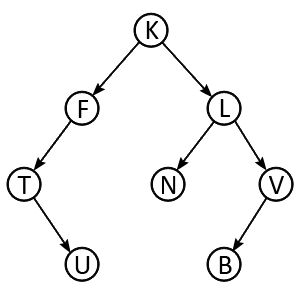
\includegraphics[height=0.3\textheight]{img/binary_tree.png}
	\caption{Пример бинарного дерева}
	\label{fig:binary_tree_example}
\end{figure}

\section{Двоичное дерево поиска}

Двоичное (или бинарное) дерево поиска (БДП) --- это бинарное дерево, обладающее следующим свойством: значение любого из узлов левого поддерева, выходящего из некоторого узла, всегда меньше значения самого узла, тогда как любой узел в правом поддереве не меньше узла~\cite{knut}.
Пример двоичного дерева поиска представлен на рисунке \ref{fig:search_tree_example}.

\begin{figure}[h]
	\centering
	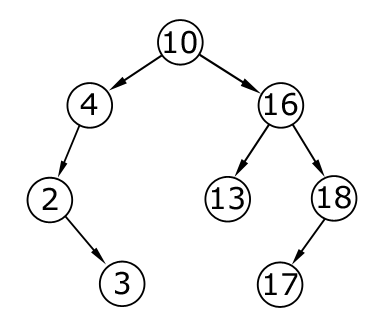
\includegraphics[height=0.3\textheight]{img/search_tree.png}
	\caption{Пример бинарного дерева поиска}
	\label{fig:search_tree_example}
\end{figure}

Основным преимуществом бинарного дерева поиска над обычным бинарным деревом является максимальное количество операций сравнения, необходимых для нахождения значения в дереве.
Максимальное количество сравнений для бинарного дерева определяется количеством узлов $N$, в то время как для бинарного дерева поиска оно определяется максимальной высотой дерева $h$, причем $h \le N$.

\section{Сбалансированное двоичное дерево поиска}

Сбалансированное двоичное дерево поиска --- это двоичное дерево поиска, в котором высота каждого из поддеревьев, имеющих общий корень, отличается не более чем на некоторую константу $k$, и при этом выполняются условия, характерные для двоичного дерева поиска.
Если $k = 1$, то такое дерево называется АВЛ-деревом.

Для узлов АВЛ-дерева определяется коэффициент сбалансированности --- разность высот правого и левого поддеревьев, принимающая одно значение из множества $\{-1, 0, 1\}$.
Ниже изображен пример АВЛ-дерева, каждому узлу которого поставлен в соответствие его реальный коэффициент сбалансированности.

\begin{figure}[h]
	\centering
	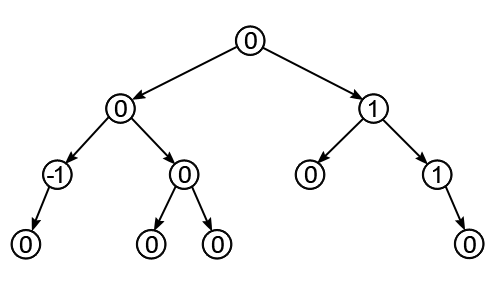
\includegraphics[height=0.3\textheight]{img/avl-tree.png}
	\caption{Пример коэффициентов сбалансированности АВЛ-дерева}
	\label{fig:avl_tree_example}
\end{figure}

Основным преимуществом АВЛ-дерева над бинарным деревом поиска является меньшее максимальное количество операций сравнения, необходимых для нахождения значения в дереве~\cite{skien}.
Так как на любом уровне $l$ АВЛ-дерева, кроме последнего, количество вершин всегда равно $2^l$, то для $N$ вершин высота дерева $h$ будет равна $\log_2 N$.
В АВЛ-дереве, как и в бинарном дереве поиска, максимальное количество сравнений ограничено высотой дерева $h$.
Из чего следует, что в АВЛ-дереве, в отличие от бинарного дерева поиска, есть ограничение на максимальное количество сравнений, необходимых для поиска значения в дереве, что может быть важно, например, при использовании рекурсии.


\section*{Вывод}

В этом разделе была представлена информация о сбалансированном и несбалансированном двоичном дереве поиска.
